\section{Further comments}

Here we provide some further tips.

\mypar{Further general guidelines}

\begin{itemize}
\item For short papers, to save space, I use paragraph titles instead of
subsections, as shown in the introduction.

\item It is generally a good idea to break sections into such smaller
units for readability and since it helps you to (visually) structure the story.

\item The above section titles should be adapted to more precisely
reflect what you do.

\item Each section should be started with a very
short summary of what the reader can expect in this section. Nothing
more awkward as when the story starts and one does not know what the
direction is or the goal.

\item Do not use subsubsections.

\item Make sure you define every acronym you use, no matter how
convinced you are the reader knows it.

\item Always spell-check before you submit.

\item Be picky. When writing a paper you should always strive for 
high quality. Many people may read it and the quality makes a big difference.
In this class, the quality contributes to the grade.

\item Books helping you to write better: \cite{Higham:98} and \cite{Strunk:00}.
\end{itemize}

\mypar{Graphics} For plots that are not images {\em never} generate (even as intermediate step)
jpeg, gif, bmp, tif. Use eps, which means encapsulate postscript, or pdf. This way it is
scalable since it is a vector graphic description of your graph. E.g.,
from Matlab, you can export to eps or pdf.

Fig.~\ref{fftperf} is an example plot that I used in a lecture. Note that the fontsize in the plot should not be any smaller. On the other hand it is also a good rule that the font size in the plot is not larger than the one in the caption (otherwise it looks ugly).

\begin{figure}\centering
  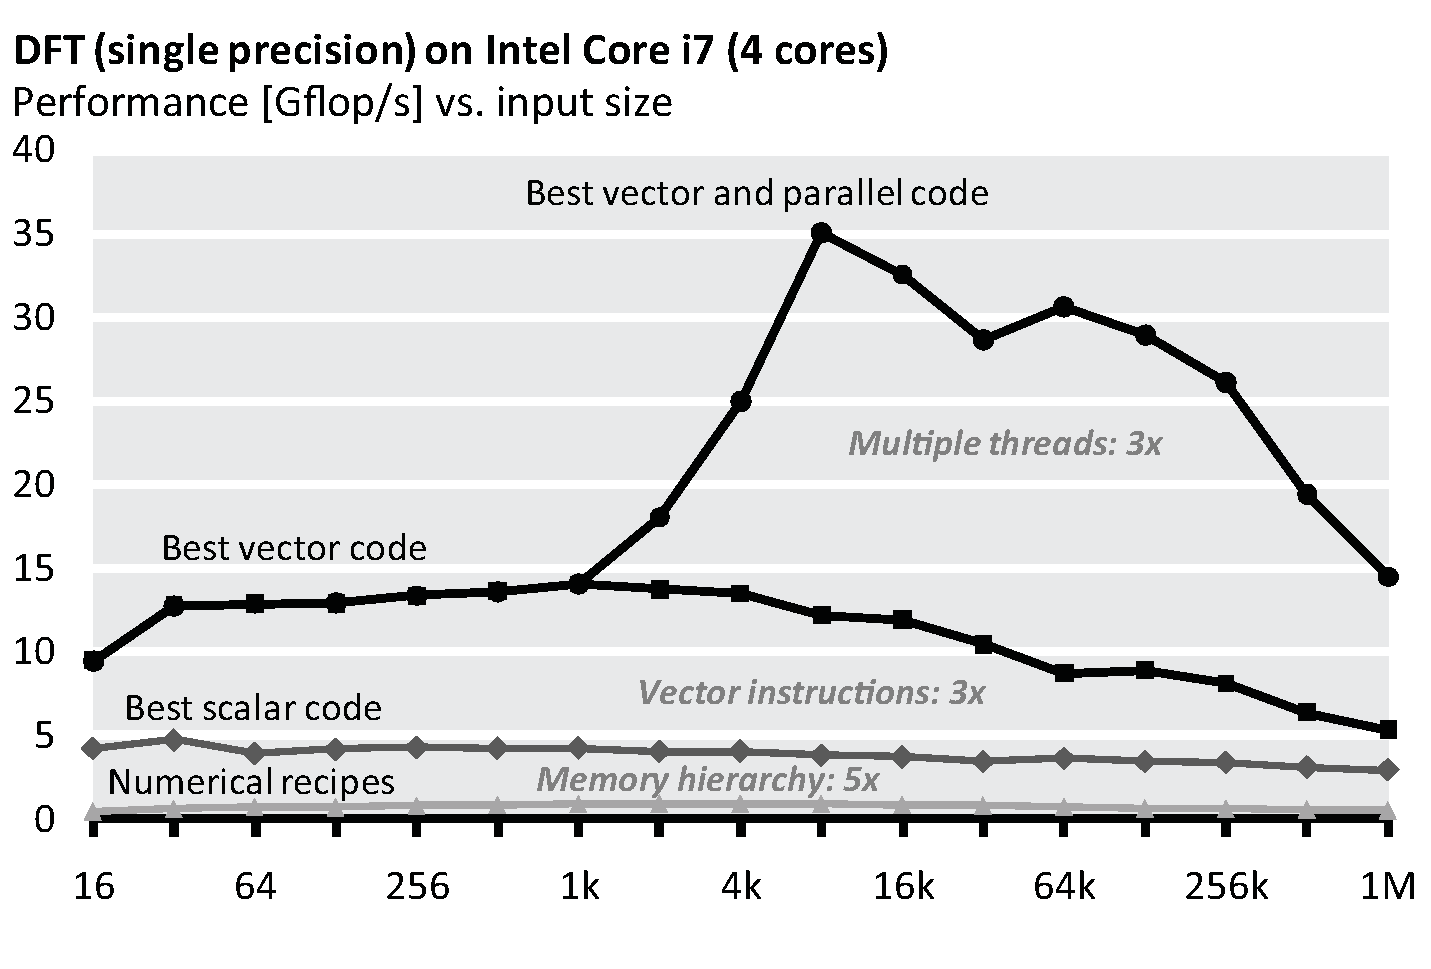
\includegraphics[scale=0.33]{dft-performance.pdf}
  \caption{Performance of four single-precision implementations of the
  discrete Fourier transform. The operations count is roughly the
  same. {\em The labels in this plot are about the smallest you should go.}\label{fftperf}}
\end{figure}

\bigskip
{\bf Up to here you have 8 pages.}

\section{Contributions of Team Members (Mandatory)}

In this mandatory section (which is not included in the 8 pages limit) each team member should very briefly (telegram style is welcome) explain what she/he did for the project. I imagine this section to be between one column and one page (absolute maximum).

Include only 
\begin{itemize}
	\item What relates to optimizing your chosen algorithm / application. This means writing actual code for optimization or for analysis.
	\item What you did before the submission of the presentation.
\end{itemize}
Do not include
\begin{itemize}
	\item Work on infrastructure and testing.
	\item Work done after the presentation took place.
\end{itemize}

Example and structure follows.

\mypar{Marylin} Focused on non-SIMD optimization for the variant 2 of the algorithm. Cache optimization, basic block optimizations, small generator for the innermost kernel (Section 3.2). Roofline plot. Worked with Cary and Jane on the SIMD optimization of variant 1, in particular implemented the bit-masking trick discussed.

\mypar{Cary} ...

\mypar{Gregory} ...

\mypar{Jane} ...
